\chapter{Preparação Dos Dados}

\section{Dado Bruto}
O modelo criado pelo sistema é baseado nos dados coletados no servidor DNS do IME. Esses dados são privados e foram coletados em diversos dias de fevereiro a abril de 2012.

Cada linha possui
\begin{itemize}
\item Data
\item Horário
\item Ip do Cliente
\item Porta do Cliente
\item URL Buscada
\item Tipo de Requisição
\item Ip do Servidor DNS
\end{itemize}

Veja em seguida um exemplo de registro de requisição extraído da base de dados

\begin{quote}
11-Mar-2012 12:24:16.772 queries: info: client 41.128.225.42\#57135: query: rEcREIo.DE9.iMe.eb.br IN A - (200.20.120.33)
\end{quote}

A extração dos dados de cada linha é feita através de uma Expressão Regular e o usuário é avisado quando o sistema falha em aplicar o filtro, seja por expressão não prevista pela Expressão Regular, seja por má formação no registro. 

Após aplicar o filtro em cada linha extraída diretamente do registro do servidor DNS do IME, o dado sanitizado é armazenado de modo amigável para a criação do modelo. O sistema salva os dados em um banco de dados PostgreSQL, mas é possível extender o armazenamento em arquivos de texto.

\section{Banco de Dados}
Previu-se que para o cálculo das características dos usuários a rapidez ao acesso das informações seria crítica para a temporização do sistema. Partindo dessa premissa, decidiu-se integrar a um Gerenciador de Banco de Dados, no caso PostgreSQL, como parte da nossa solução, para facilitar a escrita, leitura e atualização das informações coletadas dos registros DNS.

A figura \ref{fig:relational_diagram} apresenta a representação relacional do banco de dados, no qual já está incluso as características a serem analisadas como será esclarecido na sessão Levantamento das Características.

\begin{figure}
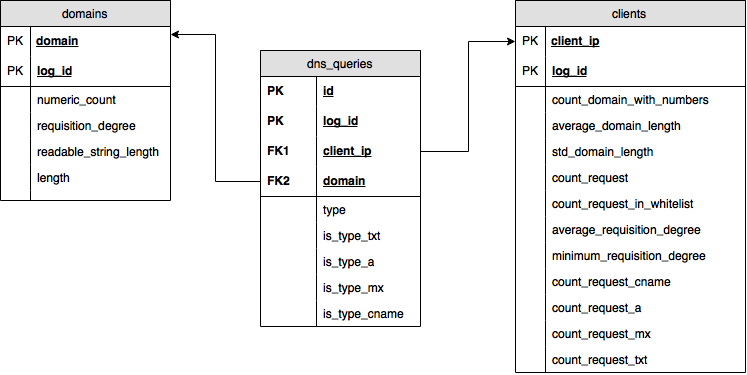
\includegraphics[width=\textwidth]{relational_diagram}
\caption[Diagrama Relacional do Sistema]{Diagrama Relacional do Sistema} \label{fig:relational_diagram}
\end{figure}

Do ponto de vista da criação do modelo, a única tabela relevante no banco de dados é a \textit{clients}, já que o sistema está preocupado em descobrir os usuários infectados. Todavia, as tabelas \textit{domains} e \textit{dns_queries} são extremamente importantes para o cálculo das características do cliente, já que elas guardam a informação de como o cliente tem se comportado na rede.

\section{Levantamento das Características}
De posse das informações apresentadas nos capítulos anteriores, é possível definir o problema que esse trabalho se propõe a resolver e, em linhas gerais, como ele será abordado.

O objetivo desse trabalho é a partir dos registros de um servidor DNS, acusar quais máquinas na rede são suspeitos de pertencer a uma botnet e merecem atenção para uma investigação. A caracterização dos IPs será feita através da análise das características da iteração que seriam.

Afim de levantar essas características três comportamentos divergentes do uso comum foram observados: a escolha dos domínios, o comportamento de máquina, os domínios visitados em comum.

\subsection{Escolha dos Domínios}
Domínios gerados automaticamente é uma prática comum entre as redes de botnets. Essa prática gera nomes provavelmente não inteligíveis podendo inclusive trazer números. Além disso, por conveniência é possível que os domínios criados tendem a ter o mesmo número caractéres. Por outro lado, apenas 7.3\% dos domínios dos um milhão primeiros domínios da Alexa contem número e que o tamanho do domínio de um usuário comum não segue nenhum padrão específico.

Não há garantia que essa feature é sempre efetiva, dado que o atacante pode gerar domínios de tamanho variável e evitar números ao gerar o domínio, por isso após a realização dos experiementos será possível confirmar ou não essa hipótese.

Para explorar essas propriedades foram propostas as seguintes caracteríticas

\begin{itemize}
\item Quantidade de consultas a domínios com alta quantidade de números
\item Média do comprimento de domínios consultados
\item Desvio Padrão dos comprimentos dos domínios consultados
\end{itemize}

\subsection{Comportamento de Máquina}

O tempo de reação de um humano a uma requisição sem sucesso não pode ser de décimos de segundo, por mera limitação de reflexo. Qualquer sinal de uso que aparente como uma máquina como essa deve ser considerada suspeita. Além disso, é possível que a máquina acabe por visitar uma quantidade de domínios maior do que o normal. Esse tipo de feature necessita ser validada, pois o comportamento de máquina pode ser mascarado.

Para explorar essas propriedades foram propostas as seguintes caracteríticas

\begin{itemize}
\item Média do intervalo entre as consultas
\item Desvio padrão dos intervalos entre consultas
\item Quantidade total de consultas realizadas
\end{itemize}

\subsection{Domínio Visitados em Comum}
Do fato de que domínios suspeitos são acessados por poucas máquinas: As botnets costumam utilizar algoritmos de geração de domínios para tentar estabelecer uma comunicação com o C\&C. Devido a isso, espera-se que os bots tentem acessar domínios que dificilmente serão procurados por máquinas normais, além do que, se a máquina infectada procura o centro de comando e controle, espera-se que muito dos domínios consultados sejam desse forma, pouco procurado por outras máquinas.

Para analisar essa propriedade, recomenda-se realizar um pré-processamento, que analisa para cada domínio consultado, por quantas máquinas diferentes ele foi consultado. Essa quantidade de máquinas que requisitou um domínio específico chamaremos de grau de requisição do domínio.

Dessa forma, acredita-se que as informações relativas ao grau dos domínios consultados pela máquina podem ser úteis para identificar um comportamento suspeito em uma máquina. Foram levantadas as seguintes característica:

\begin{itemize}
\item Grau de requisição mínimo entre os graus dos domínios consultados pela máquina
\item Média dos graus de requisição dos domínios consultados pela máquina
\item Desvio Padrão dos graus de requisição dos domínios consultados pela máquina

\end{itemize}

\subsection{Experimentos}

Não se tem garantia alguma de alteração no padrão dos tipos de consulta. Porém, esse dado é de fácil acesso e seu estudo pode evidenciar a exploração de alguma outra fragilidade nas requisições DNS.

\begin{itemize}
\item Quantidade de consultas para cada tipo de DNS
\item Porcentagem de consultas para cada tipo de DNS
\end{itemize}

Após o levantamento de todas as máquinas da rede, é feita a construção do modelo probabilístico gaussiano e de acordo após a escolha da probabilidade mínima dos exemplos normais, o sistema estará pronto para decidir se uma nova máquina poderia pertencer ou não a uma botnet.
